% THIS DOCUMENT FOLLOWS THE VOLERE TEMPLATE BY
% Suzanne Robertson and James Robertson.
% ONLY THE SECTION HEADINGS ARE PROVIDED.
%
% Risks are removed because they are covered by the Hazard Analysis.

\documentclass[12pt]{article}

\usepackage{booktabs}
\usepackage{tabularx}
\usepackage{hyperref}
\usepackage{graphicx}
\usepackage{float}
\usepackage{longtable}
\usepackage{array}
\usepackage{enumitem}
\usepackage{pdflscape}
\usepackage{amsmath}
\usepackage{amssymb}
\usepackage{caption}
\usepackage{natbib}

\setlength{\parindent}{0pt}
\setlength{\parskip}{0.35em}
\setlength{\tabcolsep}{8pt}
\renewcommand{\arraystretch}{1.15}
\setlist[itemize]{leftmargin=1.5em, itemsep=0.25em, topsep=0.35em}
\setlist[enumerate]{leftmargin=1.5em, itemsep=0.25em, topsep=0.35em}
\setlist[description]{itemsep=0.25em, topsep=0.35em}

\hypersetup{
  bookmarks=true,
  colorlinks=true,
  linkcolor=red,
  citecolor=green,
  filecolor=magenta,
  urlcolor=cyan
}

\newcommand{\lips}{\textit{Insert your content here.}}
\newcommand{\reqcard}[5]{%
\noindent\begin{tabularx}{\textwidth}{@{}p{2.35cm}X@{}}
\textbf{ID} & \textbf{#1} \\
\textbf{Requirement} & #2 \\
\textbf{Rationale} & #3 \\
\textbf{Fit Criterion} & #4 \\
\textbf{Priority} & #5 \\
\end{tabularx}\par\medskip
}

\input{../Comments}
%% Common Parts

\newcommand{\progname}{Project Proxi} % PUT YOUR PROGRAM NAME HERE
\newcommand{\authname}{Team \#23, Project Proxi
\\ Savinay Chhabra
\\ Amanbeer Singh Minhas
\\ Gourob Podder
\\ Ajay Singh Grewal} % AUTHOR NAMES                  

\usepackage{hyperref}
    \hypersetup{colorlinks=true, linkcolor=blue, citecolor=blue, filecolor=blue,
                urlcolor=blue, unicode=false}
    \urlstyle{same}
                                


\begin{document}

\title{
  Software Requirements Specification for Project Proxi
}
\author{\authname}
\date{\today}

\maketitle

~\newpage

\pagenumbering{roman}

\tableofcontents

~\newpage

\section*{Revision History}

\begin{tabularx}{\textwidth}{p{2.3cm}p{1.1cm}X}
\toprule
\textbf{Date} & \textbf{Ver.} & \textbf{Notes} \\
\midrule
10/10/2025 & 1.0 & Added initial SRS. \\
05/04/2026 & 1.1 & Added introductory text for major sections. \\
 &  & Moved repeated numeric thresholds into a symbolic constants section. \\
 &  & Rewrote project goals to be higher level. \\
 &  & Reordered glossary entries alphabetically. \\
 &  & Corrected spelling and wording issues. \\
 &  & Added rationale for key constraints. \\
 &  & Labeled assumptions as A1, A2, etc. \\
 &  & Clarified how personas affect requirement priorities. \\
 &  & Improved spacing and readability in Section 8.3. \\
 &  & Added dedicated traceability from requirements to use cases. \\
 &  & Expanded schedule and task-planning detail. \\
 &  & Added a formalized safety interaction protocol and a system state diagram subsection. \\
 
\bottomrule
\end{tabularx}

\newpage

\section{Purpose of the Project}

\subsection{User Business}
Proxi is an AI-powered desktop assistant designed to make everyday
computer use more accessible, efficient, and dependable. It allows
people to operate a computer through natural speech and text rather
than requiring every task to be completed through traditional mouse-
and keyboard-heavy workflows. The product is especially relevant for
users who face barriers with complex graphical interfaces, older adults
who benefit from simpler interaction paths, and users with temporary
or permanent accessibility needs who need more flexible control of the
desktop environment~\citep{WHODisability2023,W3CWCAG22}.

From a business perspective, Proxi addresses two closely related needs.
The first is accessibility: many users cannot consistently rely on
precise pointing, shortcut memorization, or dense interface navigation,
so a natural-language assistant can reduce friction and increase
independence. The second is productivity: even experienced users often
want faster, lower-friction workflows for repetitive desktop tasks such
as opening applications, searching for files, drafting messages, or
triggering common actions. By supporting both groups, Proxi can serve
as a practical daily-use assistant rather than a novelty interface.

Proxi's business value comes from converting user intent into safe,
traceable computer actions. Instead of forcing users to translate their
goals into technical steps, the system handles interpretation, planning,
confirmation, and execution in a way that preserves user control. This
reduces the digital divide, improves confidence for novice users, and
gives power users a more direct way to complete routine work while still
keeping destructive or risky actions visible and confirmable.

\subsection{Goals of the Project}
The goals in this subsection are intentionally high level. Quantitative
targets that serve as fit criteria are centralized in the symbolic
constants table in Section~\ref{sec:symbolic-constants} so that the
same values can be referenced consistently throughout the document.
This separation helps keep the goals stable even when implementation
details evolve, while still preserving measurable acceptance criteria in
later requirement sections. It also improves traceability by ensuring
that performance, usability, and safety thresholds are defined once and
reused uniformly across functional requirements, non-functional
requirements, and verification activities.

\begin{tabularx}{\textwidth}{p{4.1cm}X}
\textbf{G-1 (Accessibility)} & Proxi shall improve computer access for users who face barriers with keyboards, mice, and complex user interfaces. \\
\textbf{G-2 (Independent Task Completion)} & Proxi shall allow users to complete a meaningful set of everyday computer tasks through voice or text interaction. \\
\textbf{G-3 (Safety and Trust)} & Proxi shall support safe task execution through clear feedback, explicit confirmation for risky actions, and traceable results. \\
\textbf{G-4 (Usability)} & Proxi shall be simple enough for new users to learn quickly and useful enough for experienced users to adopt in everyday work. \\
\textbf{G-5 (Extensibility)} & Proxi shall provide a modular foundation that can be extended with new tools, interaction modes, and accessibility improvements. \\
\textbf{G-6 (Stretch Goals)} & Stretch goals include stronger personalization, offline support, multimodal input, and broader language coverage. \\
\end{tabularx}

\section{Naming Conventions and Terminology}
This section defines project terms, abbreviations, and shared
constants. The glossary is ordered alphabetically to improve lookup,
and the symbolic constants centralize repeated numeric thresholds so
the same values can be used consistently across goals, requirements,
and fit criteria.

\subsection{Symbolic Constants}
\label{sec:symbolic-constants}
\begin{samepage}
\vspace{-0.5\baselineskip}
This section defines the main symbolic constants used throughout this
document. These constants centralize recurring thresholds so values are
defined once and referenced consistently across goals, functional
requirements, non-functional requirements, and fit criteria. Using
symbolic names instead of repeating raw numbers also improves
maintainability: if a target changes, it can be updated in one place
without introducing inconsistencies in downstream sections.

\begingroup
\small
\setlength{\tabcolsep}{6pt}
\renewcommand{\arraystretch}{1.35}
\captionsetup{aboveskip=4pt, belowskip=4pt}
\begin{center}
\captionof{table}{Symbolic Constants}
\label{tab:symbolic-constants}
\begin{tabularx}{0.92\textwidth}{p{3.35cm}p{2.0cm}X}
\toprule
\textbf{Name} & \textbf{Value} & \textbf{Meaning} \\
\midrule
\texttt{APP\_CPU\_MAX} & 30\% &
Maximum CPU use during normal operation. \\
\texttt{APP\_LOAD\_TIME} & 200 ms &
Maximum time to load a new feature. \\
\texttt{INDOOR\_NOISE\_MAX} & 65 dB &
Moderate indoor noise limit. \\
\texttt{MOD\_NOISE\_ACC\_MIN} & 80\% &
Minimum accuracy in moderate indoor noise. \\
\texttt{QUIET\_ACC\_MIN} & 90\% &
Minimum recognition accuracy in quiet conditions. \\
\texttt{QUIET\_RESP\_MAX} & 2.0 s &
Maximum response-start time in quiet conditions. \\
\texttt{ROLLBACK\_MAX} & 60 s &
Maximum rollback time after update failure. \\
\texttt{SESS\_DURATION\_MIN} & 4 h &
Minimum continuous operation target. \\
\texttt{TASK\_SUCCESS\_MIN} & 85\% &
Minimum end-to-end task success rate. \\
\texttt{TASK\_TIME\_MAX} & 3.0 s &
Maximum time for common local actions. \\
\texttt{USER\_SAT\_MIN} & 4.0/5.0 &
Minimum usability satisfaction score. \\
\texttt{USABILITY\_GAIN\_MIN} & 20\% &
Minimum improvement over baseline workflow. \\
\bottomrule
\end{tabularx}
\end{center}
\endgroup
\end{samepage}

\subsection{Glossary of All Terms, Including Acronyms, Used by
Stakeholders Involved in the Project}

\begin{tabularx}{\textwidth}{p{3.8cm}X}
\toprule
\textbf{Term} & \textbf{Definition} \\
\midrule
\textbf{Accessibility} & Usable by people with a wide range of abilities and disabilities. \\
\textbf{Action} & A single execution of a tool with validated parameters. \\
\textbf{AI Agent} & A software agent that uses artificial intelligence to carry out tasks. \\
\textbf{Audit Log} & A record of actions taken by the system. \\
\textbf{Command} & An instruction given by the user to the system. \\
\textbf{Confirmation Gate} & An approval prompt shown before risky actions. \\
\textbf{LLM} & Large Language Model. \\
\textbf{MCP} & Model Context Protocol. \\
\textbf{MCP Client} & An AI agent that connects to an MCP server to use tools. \\
\textbf{MCP Server} & A local server that exposes tools through MCP. \\
\textbf{OS Automation Tools} & Software that allows the system to interact with the operating system. \\
\textbf{Permission Scope} & The level of access granted to the system for completing actions. \\
\textbf{PII} & Personally Identifiable Information. \\
\textbf{Plan} & An ordered sequence of actions used to fulfill a user intent. \\
\textbf{POLP} & Principle of Least Privilege. \\
\textbf{Sandbox} & A secure environment in which code can run without affecting the rest of the system. \\
\textbf{STT} & Speech-to-Text. \\
\textbf{Token} & A unit of text used by language models. \\
\textbf{TTS} & Text-to-Speech. \\
\textbf{User Interface} & The visual and interactive elements through which a user engages with the system. \\
\bottomrule
\end{tabularx}

\section{Stakeholders}
This section identifies the people and groups who influence scope,
implementation, validation, and long-term use of the product. The goal
is to make decision authority, user impact, and feedback pathways
explicit so requirement priorities remain defensible throughout the
project lifecycle.

\subsection{Client}
The clients for this project are the SFWRENG 4G06A Capstone teaching
team at McMaster University, including the course instructor and the
assigned teaching assistants.

\textbf{Role:}
They act as the academic product owners for scope, quality, and
acceptance decisions.

\textbf{Decision Authority:}
They approve major requirement changes, milestone outcomes, and final
deliverable readiness.

\textbf{Primary Success Criteria:}
The delivered system demonstrates strong accessibility alignment,
usable interaction flow, and acceptable engineering rigor for a
capstone context.

\subsection{Customer}
Our customers are the end users and organizations that will deploy
Proxi to enable inclusive and more efficient computer use:
\begin{enumerate}
  \item \textbf{Educational institutions} such as libraries, computer
  labs, and accessibility services that need dependable low-friction
  computer access support.
  \item \textbf{Healthcare and community organizations} supporting
  users with motor, vision, or hearing challenges who benefit from
  voice-first and guided interaction.
  \item \textbf{General consumers and power users} who value faster
  workflows, reduced interaction overhead, and mixed-modality control
  in daily desktop tasks.
\end{enumerate}

Across these customer groups, the most important shared outcomes are
\textbf{safe task completion}, \textbf{clear feedback}, and
\textbf{predictable behavior}.

\subsection{Other Stakeholders}
Other stakeholders include:
\begin{enumerate}
  \item \textbf{Team Proxi (development team):} Responsible for
  requirements analysis, architecture, implementation, testing,
  documentation, and integration quality.
  \item \textbf{Course staff:} Provide assessment criteria,
  risk-oriented feedback, and milestone governance.
  \item \textbf{Accessibility advisors (if engaged):} Contribute
  practical guidance on WCAG-aligned decisions and assistive-technology
  compatibility.
  \item \textbf{Pilot participants:} Provide early evidence of
  usability barriers, task-flow friction, and communication clarity.
\end{enumerate}

\subsection{Hands-On Users of the Project}
Primary hands-on users who will directly interact with Proxi:
\begin{enumerate}
  \item \textbf{Accessibility-focused users:} People with motor
  impairments or temporary and situational limitations who need
  hands-free, low-complexity, and error-tolerant interaction.
  \item \textbf{General and power users:} Users seeking faster and
  more natural workflows through voice or text, while retaining
  keyboard and mouse fallback paths.
\end{enumerate}

These groups are expected to use the same core capabilities, but they
place different emphasis on speed, guidance density, and confirmation
behavior.

\subsection{Personas}
\begin{enumerate}
  \item \textbf{P1: Amrita (72) - Elderly User}

  \textbf{Profile:}
  Amrita is a retired teacher with moderate digital literacy who uses
  her desktop for personal communication, banking, government forms,
  and telehealth appointments.

  \textbf{Primary Tasks:}
  Read and respond to email, open documents from family members,
  complete simple web forms, and join scheduled video calls.

  \textbf{Pain Points:}
  Small controls, dense interfaces, and multi-step flows increase
  cognitive load. She often loses track of where she is in a process
  and worries about making irreversible mistakes.

  \textbf{Accessibility and Usability Needs:}
  Large and readable text, plain-language prompts, explicit progress
  feedback, low-jargon error recovery, and clear confirmation before
  risky actions.

  \textbf{Success Indicators:}
  She can complete common tasks without external help, understands
  system status at each step, and confidently recovers from mistakes.

  \item \textbf{P2: Leo (21) - User with Motor Disability}

  \textbf{Profile:}
  Leo is a university student with a motor impairment that makes
  prolonged keyboard and mouse interaction painful and slow.

  \textbf{Primary Tasks:}
  Open and navigate course documents, switch between browser tabs and
  note-taking tools, draft assignment text, and manage file
  organization during study sessions.

  \textbf{Pain Points:}
  Repetitive fine-motor interactions, shortcut-heavy workflows, and
  precise cursor targeting create fatigue and reduce productivity.
  Frequent context switching further amplifies input overhead.

  \textbf{Accessibility and Usability Needs:}
  Reliable voice-first execution, complete keyboard-free coverage of
  core actions, captioned feedback, predictable command structure, and
  low-latency responses for uninterrupted work.

  \textbf{Success Indicators:}
  He can complete end-to-end coursework workflows hands-free with
  minimal corrections and without dependency on another person.

  \item \textbf{P3: Ari (28) - Power User}

  \textbf{Profile:}
  Ari is a productivity-focused knowledge worker who manages high task
  volume across spreadsheets, email, messaging, and browser-based
  systems.

  \textbf{Primary Tasks:}
  Trigger repeated multi-step workflows, retrieve files quickly,
  draft routine communications, and coordinate tasks across several
  applications in short cycles.

  \textbf{Pain Points:}
  Workflow fragmentation, repeated navigation, and command recall
  overhead interrupt concentration and reduce throughput.

  \textbf{Accessibility and Usability Needs:}
  Fast execution, concise confirmations, efficient follow-up commands,
  and reusable patterns that reduce repetitive interaction cost while
  preserving guardrails for risky operations.

  \textbf{Success Indicators:}
  He completes repeated workflows in fewer interaction steps, with
  lower context-switch overhead and sustained trust in system safety.
\end{enumerate}

\textbf{Persona Design Implication:}
The interface must balance \textbf{clarity-first interaction} for users
like Amrita and Leo with \textbf{efficiency-first flow} for users like
Ari, without compromising safety controls.

\subsection{Priorities Assigned to Users}
\textbf{Primary Priority Group:}
Accessibility-focused users, including elderly users like Amrita and
users with motor impairments like Leo. Their needs define baseline
acceptance for usability, interaction clarity, caption support, voice
control, and safety confirmation.

\textbf{Secondary Priority Group:}
General and power users like Ari. Their needs mainly influence
efficiency, reduced interaction steps, and high-frequency workflow
support after accessibility-critical requirements are satisfied.

\subsection{How Personas Affect the Requirements}
The personas directly influence requirement priorities. P1 Amrita and
P2 Leo drive the highest-priority requirements for simple language,
low-friction task completion, captions, scalable text, voice-first
operation, and explicit safety confirmation. P3 Ari mainly influences
secondary requirements related to speed, efficient task flow, and
support for repeated multi-step tasks.

In practical terms, persona influence is applied as follows:
\begin{enumerate}
  \item \textbf{P1 and P2 constraints are treated as release-critical}
  for core interaction flows.
  \item \textbf{P3-driven optimizations are treated as quality
  multipliers} once baseline accessibility and safety are satisfied.
  \item \textbf{Conflicts are resolved in favor of safety and
  accessibility} when speed and guardrails compete.
\end{enumerate}

\subsection{User Participation}
Estimated participation during the project will primarily involve end
users and the development team. Accessibility-focused users are
expected to participate for about one hour per week through remote or
in-lab sessions focused on usability testing and feedback. General
users and power users will contribute roughly one hour per week by
taking part in efficiency and performance testing of new features.

\textbf{Participation Objectives:}
Collect actionable feedback on command clarity, confirmation
understandability, error recovery flow, and end-to-end task success.

\textbf{Expected Outputs:}
Prioritized usability findings, requirement refinements, and targeted
validation scenarios for upcoming milestones.

\subsection{Maintenance Users and Service Technicians}
The primary maintenance users for this project will be the development
team. During the capstone project, they will be responsible for
identifying and fixing issues, releasing updates and patches, and
ensuring that the system continues to function as expected.

\textbf{Maintenance Scope:}
Bug triage, integration fixes, dependency upkeep, and documentation
updates for installation and troubleshooting.

\textbf{Operational Goal:}
Preserve reliability and traceability across revisions while minimizing
regression risk in accessibility and safety-critical behaviors.

\section{Mandated Constraints}
This section records external constraints and important project-level
decisions that bound the solution space. Each constraint includes a
short rationale so it is clear whether it comes from the project
context, target environment, or a team decision.

\subsection{Solution Constraints}
\reqcard{SOL-01}{The application shall run on standard consumer
hardware and shall not require specialized assistive hardware.}{The
target users are expected to use ordinary personal computers at home,
school, or work.}{The application installs and operates on ordinary
laptops or desktops with a standard microphone, speakers, display, and
keyboard.}{High}

\reqcard{SOL-02}{The application shall operate without requiring a
Proxi-specific user account or sign-up flow.}{Reducing setup friction
is important for accessibility, first-time use, and privacy.}{A user
can install and run Proxi without creating a Proxi-managed
account.}{High}

\subsection{Implementation Environment of the Current System}
\reqcard{IMECS-01}{The application shall run on mainstream desktop
operating systems such as Windows and macOS.}{These are the primary
environments available to the intended users during the capstone
project.}{The application builds and runs on supported Windows and
macOS test machines.}{High}

\reqcard{IMECS-02}{The application shall rely on standard input and
output devices such as microphones, speakers, keyboards, and
displays.}{The product is intended to be deployable without extra
equipment.}{All core user flows are executable using only standard
desktop peripherals.}{High}

\reqcard{IMECS-03}{The implementation may depend on a web-based or
JavaScript-based application stack and on MCP-compatible libraries when
this simplifies delivery.}{This is a team design decision for
implementation speed and ecosystem support, not a client-mandated
constraint.}{The selected implementation stack supports the required
Proxi features within the project timeline.}{Medium}

\subsection{Partner or Collaborative Applications}
\reqcard{PCA-01}{The application may use external AI services through
secure APIs for natural-language understanding, planning support, and
response generation.}{External AI services can improve language
coverage and implementation speed while preserving modularity.}{When
enabled, external AI calls use secure transport and return
task-relevant outputs that integrate with the local execution
flow.}{Medium}

\reqcard{PCA-02}{Integration with external accessibility tools,
including screen readers and related assistive technologies, may be
supported to improve usability for older adults and users with
disabilities.}{Compatibility with existing assistive ecosystems reduces
adoption barriers and improves inclusiveness.}{Supported workflows do
not block core interactions when common assistive tools are active on
target platforms.}{Medium}

\subsection{Off-the-Shelf Software}
\reqcard{OTSS-01}{MCP-compatible infrastructure shall be used to
provide modular tool discovery, invocation, and interface
coordination.}{Using MCP-compatible components improves extensibility
and reduces custom integration overhead.}{Tools are registerable and
invokable through the selected MCP integration path in the working
build.}{High}

\reqcard{OTSS-02}{Off-the-shelf JavaScript libraries and frameworks
shall be used where appropriate to implement interactive elements and
handle input and output operations.}{Mature libraries accelerate
development and reduce implementation risk for standard interaction
patterns.}{Core UI and interaction flows are implemented using
maintained third-party components with project-appropriate
licenses.}{High}

\reqcard{OTSS-03}{Off-the-shelf LLM services may be used for
natural-language responses and reasoning capabilities; no specialized
model training is required for baseline scope.}{Pretrained LLM
services are sufficient for capstone-level baseline intent handling and
response generation.}{Baseline intent interpretation and response
quality meet the relevant functional and usability targets without
custom model training.}{Medium}

\subsection{Anticipated Workplace Environment}
\reqcard{AWE-01}{The application is expected to run on users' personal
computers in homes, schools, offices, and assisted-living
facilities.}{The deployment context is primarily everyday desktop
environments, not specialized labs.}{Core workflows execute in
representative home, school, and office test environments on supported
desktop systems.}{High}

\reqcard{AWE-02}{The application shall be usable primarily on Windows
and macOS operating systems.}{These operating systems represent the
primary target environments for project users.}{Core features are
demonstrated and validated on supported versions of Windows and
macOS.}{High}

\reqcard{AWE-03}{The system shall support users with limited technical
experience, including older adults and people with disabilities,
through a simple and intuitive interaction model.}{Ease of
understanding is essential for inclusive adoption and safe
use.}{Usability sessions with novice and accessibility-focused users
show completion of representative tasks with minimal facilitator
support.}{High}

\reqcard{AWE-04}{The application shall function on standard consumer
computers with varying screen sizes, input methods, and processing
power, without requiring specialized hardware.}{Hardware variability is
expected in the target user population.}{Core functionality remains
available across representative low- to mid-range desktop hardware
profiles.}{Medium}

\reqcard{AWE-05}{Because background noise and poor acoustics can reduce
voice performance, the application shall provide alternative input
paths, including text and on-screen controls, when voice input is
infeasible.}{Reliable fallback input is required to preserve task
continuity in non-ideal listening conditions.}{Representative tasks
remain completable through non-voice input during noise-degraded test
scenarios.}{High}

\subsection{Schedule Constraints}
Development will follow the planned project timeline while giving
earlier attention to the highest-priority accessibility, safety, and
core-task features. Table~\ref{tab:proj-schedule} summarizes the main
external milestones.

\begin{table}[H]
\centering
\caption{Project Timeline}
\label{tab:proj-schedule}
\begin{tabularx}{\textwidth}{p{6.6cm}X}
\toprule
\textbf{Deliverable} & \textbf{Deadline} \\
\midrule
Req. Doc. and Hazard Analysis Revision 0 & October 6, 2025 \\
V\&V Plan Revision 0 & October 27, 2025 \\
Design Document Revision -1 & November 10, 2025 \\
Design Document Revision 0 & January 19, 2026 \\
Revision 0 Demonstration & February 13, 2026 \\
V\&V Report and Extras Revision 0 & March 9, 2026 \\
Final Demonstration (Revision 1) & March 29, 2026 \\
Final Documentation (Revision 1) & April 6, 2026 \\
EXPO Demonstration & April 7, 2026 \\
\bottomrule
\end{tabularx}
\end{table}

\subsection{Budget Constraints}
The project budget is limited to \$500 in total expenditure. Of this,
\$125 will be provided by the CAS department for approved expenses.

\subsection{Enterprise Constraints}
There are no enterprise constraints beyond the need to satisfy course
requirements and academic policies. The application may use any
service or LLM as required as long as it adheres to the budget
constraints.

\section{Relevant Facts and Assumptions}
This section separates established project facts, business rules, and
explicit assumptions. Assumptions are labeled so they can be
referenced by design, testing, and later revisions.

\subsection{Relevant Facts}
\begin{enumerate}
  \item Proxi's main goal is to enable hands-free computer control
  through natural language commands for disabled users while also
  supporting users who want a more efficient workflow.
  \item The system will run on desktop operating systems such as
  Windows and macOS and will interact with common applications such as
  web browsers, file browsers, calendar tools, and email tools.
  \item Some actions can be high risk, such as deleting files or
  changing system settings, so the system must confirm with the user
  before performing such actions.
\end{enumerate}

\subsection{Business Rules}
Proxi must get user consent before accessing or handling personal data.
It must minimize the amount of data shared with external services and
send only what is strictly needed to fulfill the user's request. Any
command that involves high risk, such as deleting data or changing
system settings, must be confirmed before execution. All actions
should be recorded in an audit log so that incorrect actions can be
traced and, when possible, reversed. Tools may operate only within the
permission scope explicitly granted by the user.

\subsection{Assumptions}

\noindent\textbf{A1 (Hardware)} \\
The user has a working computer with a microphone and audio output and
can run the software on a modern desktop operating system.

\noindent\textbf{A2 (Permissions)} \\
The user can grant the permissions needed by the system, including
microphone, accessibility, or automation permissions.

\noindent\textbf{A3 (Internet)} \\
The user has a reliable internet connection when using features that
depend on remote LLM or web services.

\noindent\textbf{A4 (Environment and Language)} \\
The user is in an environment where the microphone can capture speech
clearly and will speak in a supported language.

\noindent\textbf{A5 (Off-the-Shelf Model Adequacy)} \\
An off-the-shelf LLM is assumed to be adequate for the baseline
command-understanding tasks in scope. This assumption will be checked
through verification activities tied to functional accuracy, task
success, and usability.

\section{The Scope of the Work}
This section describes the current problem context, the project's role
within that context, the high-level partitioning of the work, and the
main business use case that motivates the product.

\subsection{The Current Situation}
Desktop computing still assumes that users can reliably navigate dense
graphical interfaces, operate precise pointer controls, and remember
multi-step interaction paths. For many users, this assumption does not
hold in everyday practice.

\textbf{Current Barriers:}
\begin{itemize}
  \item Users with motor impairments or temporary mobility limits may
  find keyboard and mouse interaction slow, fatiguing, or infeasible.
  \item Elderly and novice users can struggle with interface complexity,
  hidden settings, and jargon-heavy error messages.
  \item Voice assistants commonly used today provide limited
  task-execution depth for desktop workflows and often stop at shallow
  command handling.
\end{itemize}

As a result, many users cannot complete routine digital tasks with
consistent independence, speed, and confidence. This creates a clear
need for an assistant that is not only conversational, but also
operationally useful across real desktop tasks.

\subsection{The Context of the Work}
This project addresses the above gap by building an AI-powered,
desktop-oriented assistive platform that converts natural-language
intent into safe and traceable computer actions.

\textbf{Project Positioning:}
\begin{itemize}
  \item Proxi acts as an \textbf{intermediary layer} between the user
  and the operating environment.
  \item It accepts \textbf{speech and text input}, interprets intent,
  plans executable steps, and invokes tools through a modular
  integration model.
  \item It emphasizes \textbf{accessible interaction} and
  \textbf{safety-aware execution}, including explicit confirmation for
  risky actions and clear user feedback.
\end{itemize}

Within the scope of this capstone, the work focuses on practical
desktop task support (for example opening applications, navigating
files, and handling common communication workflows) rather than
building full replacements for third-party software. This keeps the
solution applicable, testable, and aligned with project constraints.

\subsection{Work Partitioning}
The work is partitioned into six coordinated workstreams so design,
implementation, and validation can proceed in parallel while remaining
traceable to requirements.

\begin{enumerate}
  \item \textbf{Input and Recognition Layer}

  Captures user requests through voice and text channels and normalizes
  them into a consistent input format for downstream processing.

  \item \textbf{Natural Language Understanding Layer}

  Interprets normalized input, resolves intent and entities, and
  produces structured task representations suitable for planning.

  \item \textbf{Planning and Execution Layer}

  Generates safe execution plans and invokes modular tools to perform
  user-requested desktop actions within configured permission scope.

  \item \textbf{Feedback and Output Layer}

  Communicates status, confirmations, errors, and outcomes through
  readable text and optional speech, with emphasis on clarity and
  recoverability.

  \item \textbf{Accessibility and Usability Design}

  Defines interaction constraints and interface behavior for inclusive
  use, including readability, low-friction controls, and
  confirmation-oriented safety design.

  \item \textbf{Evaluation and Testing}

  Verifies functional correctness, usability, performance, and safety
  behavior through scenario-based testing, stakeholder feedback, and
  milestone-aligned validation activities.
\end{enumerate}

Together, these workstreams establish a clear delivery path from user
input to validated task outcomes while preserving modularity for future
extension.

\subsection{Specifying a Business Use Case (BUC)}
\textbf{BUC-01: Intelligent Accessibility Assistant}

\noindent\textbf{Primary Actor:}
User with limited mobility, low computer literacy, or hands-busy use.

\noindent\textbf{Supporting Actors:}
Operating system services, desktop applications, and connected tool
integrations invoked through Proxi.

\noindent\textbf{Goal:}
Complete desktop tasks through natural speech or text with minimal
manual navigation while preserving user safety and control.

\noindent\textbf{Trigger:}
The user issues a request in voice or text, for example
``Open my email and draft a message to my doctor.''

\noindent\textbf{Preconditions:}
\begin{itemize}
  \item The user has access to a supported device with microphone,
  speakers, and input fallback options.
  \item The assistive system is installed, running, and has the
  required permissions for the requested action.
  \item If applicable, network connectivity is available for remote
  services used by the request.
\end{itemize}

\noindent\textbf{Main Success Scenario:}
\begin{enumerate}
  \item The user submits a request using voice or text.
  \item The system captures and normalizes the input.
  \item The system identifies intent and required entities.
  \item The system generates a task plan using available tools.
  \item For risky actions, the system requests explicit confirmation.
  \item The system executes the approved plan.
  \item The system reports outcome status and next-step guidance in
  plain language (with speech and text when enabled).
  \item The system records interaction and execution events for
  traceability.
\end{enumerate}

\noindent\textbf{Extensions and Exception Flows:}
\begin{itemize}
  \item \textbf{E1 - Ambiguous Request:} The system asks a concise
  clarification question and resumes planning after user disambiguation.
  \item \textbf{E2 - Missing Permission or Tool Access:} The system
  stops execution, explains the blocker, and provides corrective steps.
  \item \textbf{E3 - High-Risk Action Denied:} The system cancels the
  risky step, confirms no destructive change was made, and offers safe
  alternatives.
  \item \textbf{E4 - Execution Failure:} The system reports failure
  cause, logs diagnostic context, and suggests retry or fallback action.
\end{itemize}

\noindent\textbf{Success Guarantee (Postconditions on Success):}
\begin{itemize}
  \item Requested task is completed or progressed to a valid next step.
  \item User receives clear completion feedback and any relevant
  follow-up options.
  \item Audit trail entries are persisted for command, plan, and
  outcome events.
\end{itemize}

\noindent\textbf{Minimal Guarantee (Postconditions on Failure):}
\begin{itemize}
  \item No unconfirmed destructive action is executed.
  \item The user receives an understandable failure message and
  recovery guidance.
  \item Failure context is logged for support and debugging.
\end{itemize}

\noindent\textbf{Business Value:}
This use case operationalizes inclusive, low-friction computer control
by converting natural-language intent into safe, traceable desktop
actions across everyday workflows.

\section{Business Data Model and Data Dictionary}
This section defines the core business entities and their main
attributes. Figure~\ref{fig:business-data-model} presents the business
data model, and the subsequent tables define each entity.

\subsection{Business Data Model}
\begin{figure}[H]
  \centering
  \includegraphics[width=0.88\textwidth]{Business_Model.png}
  \caption{Business Data Model}
  \label{fig:business-data-model}
\end{figure}

\subsection{Data Dictionary}

\subsubsection*{User}
\noindent\begin{tabularx}{\textwidth}{@{} l l X @{}}
\toprule
\textbf{Attribute} & \textbf{Type} & \textbf{Description} \\
\midrule
userId & UUID & Unique identifier for a user \\
displayName & String & Name shown in confirmations or UI \\
role & Enum & Authorization role \\
\bottomrule
\end{tabularx}\par\medskip

\subsubsection*{Session}
\noindent\begin{tabularx}{\textwidth}{@{} l l X @{}}
\toprule
\textbf{Attribute} & \textbf{Type} & \textbf{Description} \\
\midrule
sessionId & UUID & Logical dialog or control session \\
startedAt / endedAt & Timestamp & Session start and end \\
status & Enum & Active, Ended, or Error \\
\bottomrule
\end{tabularx}\par\medskip

\subsubsection*{Command}
\noindent\begin{tabularx}{\textwidth}{@{} l l X @{}}
\toprule
\textbf{Attribute} & \textbf{Type} & \textbf{Description} \\
\midrule
commandId & UUID & Captured user request \\
modality & Enum & Voice, Text, or Mixed \\
rawText & String & Transcribed or typed command text \\
timestamp & Timestamp & Capture time \\
\bottomrule
\end{tabularx}\par\medskip

\subsubsection*{Intent}
\noindent\begin{tabularx}{\textwidth}{@{} l l X @{}}
\toprule
\textbf{Attribute} & \textbf{Type} & \textbf{Description} \\
\midrule
intentId & UUID & Normalized goal \\
name & String & Intent label \\
confidence & Float & Classifier confidence \\
\bottomrule
\end{tabularx}\par\medskip

\subsubsection*{Plan}
\noindent\begin{tabularx}{\textwidth}{@{} l l X @{}}
\toprule
\textbf{Attribute} & \textbf{Type} & \textbf{Description} \\
\midrule
planId & UUID & Ordered set of actions \\
summary & String & One-line description \\
status & Enum & Proposed, Running, Succeeded, Failed \\
\bottomrule
\end{tabularx}\par\medskip

\subsubsection*{Action}
\noindent\begin{tabularx}{\textwidth}{@{} l l X @{}}
\toprule
\textbf{Attribute} & \textbf{Type} & \textbf{Description} \\
\midrule
actionId & UUID & Atomic operation \\
toolId & UUID & Tool to invoke \\
parameters & JSON & Tool inputs \\
result & JSON & Tool outputs or return value \\
riskLevel & Enum & Low, Medium, or High \\
\bottomrule
\end{tabularx}\par\medskip

\subsubsection*{Tool}
\noindent\begin{tabularx}{\textwidth}{@{} l l X @{}}
\toprule
\textbf{Attribute} & \textbf{Type} & \textbf{Description} \\
\midrule
toolId & UUID & Unique tool capability \\
name & String & Human-friendly tool name \\
description & String & Purpose and constraints \\
isDestructive & Boolean & Writes, installs, or deletes \\
\bottomrule
\end{tabularx}\par\medskip

\subsubsection*{AuditLog}
\noindent\begin{tabularx}{\textwidth}{@{} l l X @{}}
\toprule
\textbf{Attribute} & \textbf{Type} & \textbf{Description} \\
\midrule
auditId & UUID & Append-only log entry \\
eventType & Enum & Example: CommandCaptured, ActionSucceeded \\
details & String/JSON & Minimal facts about the event \\
createdAt & Timestamp & When the entry was written \\
\bottomrule
\end{tabularx}\par\medskip

\section{The Scope of the Product}
This section defines the product boundary and summarizes the main ways
in which users will interact with the system. The use cases in this
section describe the major user-visible capabilities that motivate the
functional requirements in Section~9.

\subsection{Product Boundary}
Proxi is an assistive desktop orchestration layer that enables users
to perform common computer tasks through natural speech or text. It
translates user intent into safe, scoped actions and provides clear
feedback before, during, and after execution.

\textbf{Boundary Definition:}
The product coordinates supported actions across the existing desktop
environment; it does not replace full third-party applications.

\textbf{In-Scope Features:}
\begin{itemize}
  \item Multi-modal input capture and interpretation (voice and text).
  \item Desktop action execution through MCP-compatible tool
  integrations.
  \item Safety guardrails, including confirmation before risky or
  destructive operations.
  \item Accessible system feedback through text, speech, or both.
  \item Short-term session context and local audit logging for
  traceability.
\end{itemize}

\textbf{Out-of-Scope Features:}
\begin{itemize}
  \item Full replacement of third-party tools such as complete email
  clients, browsers, or office suites.
  \item Unattended remote administration or unsupervised control of
  user systems.
  \item Enterprise-scale policy governance and organization-wide IT
  management.
  \item Default long-term cloud retention of user interaction data.
\end{itemize}

\subsection{Product Use Case Table}
Table~\ref{tab:puc-table} summarizes the main product use cases.

\begin{table}[H]
\centering
\caption{Product Use Case Table}
\label{tab:puc-table}
\begin{tabular}{|p{2.7cm}|p{2.1cm}|p{3.2cm}|p{3.2cm}|p{2.6cm}|}
\hline
\textbf{Use Case} &
\textbf{Actors} &
\textbf{Description} &
\textbf{Preconditions} &
\textbf{Outcome} \\
\hline
PUC-01: Open Application &
User &
Open a named app. &
App installed; automation allowed. &
App launched or focused. \\
\hline
PUC-02: Open and Read File &
User &
Open a file; preview or read. &
File exists; within scope. &
File opened; content visible. \\
\hline
PUC-03: Browse and Search &
User &
Go to a URL or search. &
Browser available; internet on. &
Page or results shown. \\
\hline
PUC-04: Draft Message or Email &
User &
Create a short draft. &
Mail or editor available. &
Draft opens prefilled. \\
\hline
PUC-05: Save or Organize File &
User &
Save As, move, or rename. &
Paths allowed; confirm overwrite. &
Operation completed. \\
\hline
PUC-06: Interact with Open App &
User &
Perform simple in-app actions. &
Target app open; allowed scope. &
Action done or reason shown. \\
\hline
\end{tabular}
\end{table}

\subsection{Individual Product Use Cases (PUC's)}
This subsection expands each product use case with concise behavioral
detail to support design alignment and test planning.

\medskip
\noindent\textbf{PUC-01: Open Application}

\textbf{Intent:} Open or focus a named application quickly.

\textbf{Behavior:} Proxi resolves candidate matches, requests
disambiguation if needed, validates execution scope, and opens or
focuses the selected app.

\textbf{Result:} The requested application becomes available and a
clear success message is returned.

\medskip
\noindent\textbf{PUC-02: Open and Read File}

\textbf{Intent:} Access and review file contents with minimal manual
navigation.

\textbf{Behavior:} Proxi resolves file identity within allowed scope,
opens it in the default viewer, and can optionally provide readback or
short summary assistance.

\textbf{Result:} The user can inspect target content and continue with
follow-up tasks.

\medskip
\noindent\textbf{PUC-03: Browse and Search}

\textbf{Intent:} Navigate to a destination or find information on the
web.

\textbf{Behavior:} Proxi validates user input as URL or query, launches
the browser path, and requests confirmation when destinations appear
risky or ambiguous.

\textbf{Result:} The correct page or search results are displayed with
clear status feedback.

\medskip
\noindent\textbf{PUC-04: Draft Message or Email}

\textbf{Intent:} Produce communication drafts from natural-language
instructions.

\textbf{Behavior:} Proxi extracts recipient and message details, opens
the draft surface in the chosen application, and pre-fills content for
user review.

\textbf{Result:} An editable draft is created, with final send control
remaining with the user.

\medskip
\noindent\textbf{PUC-05: Save or Organize File}

\textbf{Intent:} Complete common file organization tasks safely.

\textbf{Behavior:} Proxi validates paths and operation type, handles
conflicts (for example name collisions), and requests confirmation for
overwrite or destructive impact.

\textbf{Result:} Requested file-state changes are completed safely or a
clear blocker is reported.

\medskip
\noindent\textbf{PUC-06: Interact with Open App}

\textbf{Intent:} Perform focused actions inside an already-open
application.

\textbf{Behavior:} Proxi executes simple in-app operations (select,
click, type, toggle) and asks follow-up questions when intent is
underspecified.

\textbf{Result:} The target action is completed or failure is explained
with a suggested next step.

\subsection{System State Diagram}
The following state model captures the critical safety-oriented flow of
a Proxi interaction. This visual specification complements the formal
interaction protocol in Section~9.3.

\begin{figure}[H]
  \centering
  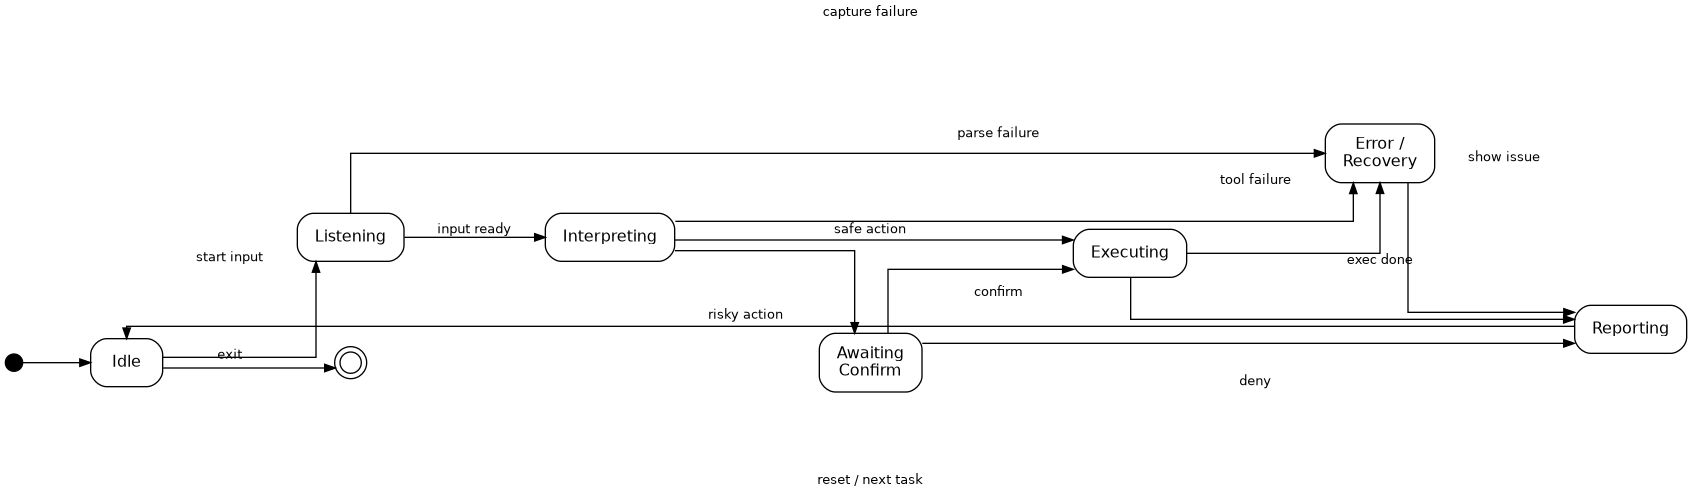
\includegraphics[width=1.0\textwidth,height=0.42\textheight]{StateDiagram.png}
  \caption{System State Diagram}
  \label{fig:state-diagram}
\end{figure}

\section{Functional Requirements}
This section states what the system does. To preserve traceability with
the existing design and V\&V documents, the requirement identifiers are
kept the same even where the wording has been refined.

\subsection{Functional Requirements}

\reqcard{FUNC.R.1}{The system shall accept user input through both
speech and text interfaces.}{Proxi must support hands-free
accessibility use and fallback text interaction for noisy or
inaccessible environments.}{Supported voice and text commands are
accepted and passed into the processing pipeline during system
testing.}{High}

\reqcard{FUNC.R.2}{The system shall convert speech input into text
using an automatic speech recognition module.}{Speech input must be
normalized into text before intent interpretation.}{Speech input is
converted into text suitable for downstream intent
processing.}{High}

\reqcard{FUNC.R.3}{The system shall interpret user intent from natural
language input to determine the desired task.}{The system must
determine what task the user wants without requiring technical
commands.}{Natural-language requests are mapped to a structured intent
for the task planner.}{High}

\reqcard{FUNC.R.4}{The system shall create and execute a plan that
invokes one or more tools on behalf of the user.}{User-visible task
completion depends on safe composition of lower-level actions.}{The
system achieves at least \texttt{TASK\_SUCCESS\_MIN} successful
completion on representative end-to-end task scenarios.}{High}

\reqcard{FUNC.R.5}{The system shall present task status and task
results to the user in text, speech, or both.}{Users need continuous
feedback to understand what the system is doing.}{Each executed command
produces a user-visible status or result message.}{High}

\reqcard{FUNC.R.6}{The system shall maintain short-term session context
so that users can issue follow-up commands.}{Natural interaction
requires short follow-up references such as ``that'' or ``the last
one.''}{Follow-up references to recent entities or actions are resolved
using session context.}{Medium}

\reqcard{FUNC.R.7}{The system shall log user interactions and task
results for traceability and debugging.}{Traceability is needed for
debugging, auditing, and future improvement.}{Each user session
produces timestamped log entries for commands, plans, and
outcomes.}{Medium}

\reqcard{FUNC.R.8}{The system shall allow users to complete supported
tasks without requiring low-level system interfaces such as raw file
paths or command-line tools.}{The product goal is high-level
accessible control, not low-level system administration.}{Users can
complete supported tasks through the Proxi interface without needing
raw OS commands or internal file-system knowledge.}{High}

\reqcard{FUNC.R.9}{The system shall request explicit confirmation
before executing privileged or destructive actions.}{Risky tasks must
not execute silently.}{Each privileged or destructive action triggers a
confirmation step before execution.}{High}

\subsection{Traceability Summary}
Table~\ref{tab:persona-traceability} summarizes how the highest
priority personas and goals map to the main requirement categories.

\begin{table}[H]
\centering
\caption{Persona and Goal Traceability Matrix}
\label{tab:persona-traceability}
\begin{tabularx}{\textwidth}{p{2cm}p{4.6cm}X}
\toprule
\textbf{Source} & \textbf{Main Need} &
\textbf{Primary Requirement Links} \\
\midrule
P1 Amrita &
Clear feedback, low complexity, readable interface &
EOU.R.1--EOU.R.3, UAP.R.1--UAP.R.3, ACC.R.2,
APP.1--APP.5 \\
P2 Leo &
Hands-free control, captions, accessible workflows &
FUNC.R.1--FUNC.R.9, ACC.R.1--ACC.R.2,
SAF.R.1--SAF.R.2 \\
P3 Ari &
Efficient repeated workflows and fast task completion &
FUNC.R.4--FUNC.R.8, SAL.R.1--SAL.R.2,
SOE.R.1--SOE.R.2 \\
G-1 &
Accessibility &
ACC.R.1--ACC.R.2, EOU.R.1--EOU.R.3,
APP.1--APP.5 \\
G-2 &
Independent task completion &
FUNC.R.1--FUNC.R.9, POA.R.1--POA.R.2,
SAL.R.1--SAL.R.2 \\
G-3 &
Safety and trust &
SAF.R.1--SAF.R.2, UAP.R.2--UAP.R.3,
ROFT.R.1--ROFT.R.2 \\
\bottomrule
\end{tabularx}
\end{table}

\subsection{Formalization of Interaction Safety Protocol}
A critical portion of the system is the user-command execution flow for
potentially risky actions. Proxi shall follow the state machine below.

Let
\[
S =
\{ Idle, Listening, Interpreting, AwaitingConfirm, Executing, Reporting
\}.
\]

Let
\[
E =
\{ startInput, inputReady, intentReady, risky, confirm, deny,
execDone, reset \}.
\]

Let
\[
\delta : S \times E \rightarrow S.
\]

The required transitions are:
\[
\delta(Idle, startInput) = Listening
\]
\[
\delta(Listening, inputReady) = Interpreting
\]
\[
\delta(Interpreting, intentReady) = Executing
\]
\[
\delta(Interpreting, risky) = AwaitingConfirm
\]
\[
\delta(AwaitingConfirm, confirm) = Executing
\]
\[
\delta(AwaitingConfirm, deny) = Reporting
\]
\[
\delta(Executing, execDone) = Reporting
\]
\[
\delta(Reporting, reset) = Idle
\]

Safety invariant:
\[
\forall a \in RiskyActions :
Execute(a) \Rightarrow Confirmed(a)
\]

This invariant states that any risky action may execute only after an
explicit confirmation event has been observed.

\section{Look and Feel Requirements}
This section describes the intended visual style and presentation of
the system. These requirements guide interface consistency and are
supported by the usability and accessibility requirements that follow.

\subsection{Appearance Requirements}
\reqcard{APP.1}{The interface shall look simple and familiar, like a
normal desktop tool with a clear status area that shows when the
system is listening, thinking, or ready.}{Users should understand the
current system state at a glance.}{The main interface visibly displays
system state in all tested interaction modes.}{High}

\reqcard{APP.2}{Main actions such as listen, stop, undo, and confirm
shall be clearly visible as controls on the main screen.}{Critical
controls must be discoverable without deep navigation.}{All critical
controls are accessible within one main view.}{High}

\reqcard{APP.3}{The interface shall avoid clutter and show only the
most important options by default.}{Minimalism reduces cognitive
load.}{Advanced settings are separated from the main interaction
flow.}{Medium}

\reqcard{APP.4}{Text and buttons shall be large enough to be easy to
read and select.}{Large text and controls support elderly and
low-vision users.}{The interface remains usable at 200\% text
scaling.}{High}

\reqcard{APP.5}{A light and dark theme option shall be
available.}{Users have different comfort and visibility
preferences.}{Users can switch between light and dark themes without
loss of functionality.}{Low}

\subsection{Style Requirements}
\reqcard{STY.1}{Labels and messages shall use short, plain language
with no unnecessary technical jargon.}{The target users should not
need specialist knowledge to understand system feedback.}{Reviewed
messages avoid internal or tool-specific jargon in user-facing
flows.}{High}

\reqcard{STY.2}{When the system speaks, the same content shall also
appear on screen as captions.}{Captions improve accessibility and
reinforce spoken feedback.}{All spoken responses have matching
on-screen text.}{High}

\reqcard{STY.3}{Icons shall be consistent and paired with short text
labels.}{Text labels reduce ambiguity in icon
interpretation.}{Primary icons used in the interface have
corresponding labels.}{Medium}

\section{Usability and Humanity Requirements}
This section captures how approachable, learnable, understandable, and
accessible the system should be for the target users identified
earlier.

\subsection{Ease of Use Requirements}
\reqcard{EOU.R.1}{The system shall be easy for new users to start
using.}{Low-friction onboarding is necessary for
accessibility-focused users.}{Basic tasks such as opening an
application or reading a file require only one simple command or
button press in typical flows.}{High}

\reqcard{EOU.R.2}{The system shall have an intuitive interface that
does not overwhelm users.}{Users should not struggle to find core
actions.}{Main actions such as listen, stop, undo, and confirm are
clearly visible and easy to access.}{High}

\reqcard{EOU.R.3}{After a short introduction, users should be able to
complete most everyday tasks without assistance.}{The system should
become useful quickly in real use.}{Task effectiveness improves by at
least \texttt{USABILITY\_GAIN\_MIN} over a baseline workflow.}{High}

\subsection{Personalization and Internationalization Requirements}
\reqcard{PER.R.1}{The system shall adapt to a user's speech patterns
over time to improve recognition quality.}{Repeated use should reduce
friction for frequent users.}{The system stores and applies allowed
local personalization settings.}{Medium}

\reqcard{PER.R.2}{The system shall support Canadian English standards
for language, date, and time formatting and allow future localization
if needed.}{The project is developed in a Canadian academic
context.}{Default language and formatting reflect Canadian English
conventions.}{Medium}

\subsection{Learning Requirements}
\reqcard{LEA.R.1}{The system shall have a short learning curve,
allowing new users to understand and use basic commands
quickly.}{The first-use experience should not require formal
training.}{New users can understand the basic interaction model within
a short guided introduction.}{High}

\reqcard{LEA.R.2}{The system shall provide a list of example commands
or a ``What can I say?'' help option.}{Users need discoverable
examples to build confidence.}{Example commands are accessible through
the interface during use.}{High}

\subsection{Understandability and Politeness Requirements}
\reqcard{UAP.R.1}{The system shall use simple and clear language for
all user-facing messages.}{Clarity reduces user confusion and error
recovery time.}{User-facing messages avoid unexplained technical
terminology.}{High}

\reqcard{UAP.R.2}{The system shall confirm actions that could change
or delete important files or settings before executing them.}{Clear
confirmation protects user trust and data.}{All destructive or
privileged actions trigger explicit confirmation.}{High}

\reqcard{UAP.R.3}{Error messages shall be polite, explain the issue in
plain language, and suggest a next step.}{Helpful error recovery is
part of usable accessibility support.}{Tested error messages include
cause and suggested recovery step.}{Medium}

\subsection{Accessibility Requirements}
\reqcard{ACC.R.1}{The system shall allow all core actions, including
setup and exit, to be performed using voice commands without requiring
a keyboard or mouse.}{Hands-free control is a core accessibility
goal.}{Core actions are completable through the voice-only path during
testing.}{High}

\reqcard{ACC.R.2}{The system shall comply with recognized
accessibility standards such as WCAG 2.2 and AODA where applicable to
the interface.}{The system should follow established accessibility
guidance rather than ad hoc design choices.}{The interface provides
captions for spoken responses, supports text scaling, and ensures
sufficient contrast in tested views.}{High}

\section{Performance Requirements}
This section defines quantitative expectations for latency, accuracy,
fault tolerance, and capacity. Where possible, the fit criteria are
expressed using the symbolic constants from
Table~\ref{tab:symbolic-constants}.

\subsection{Speed and Latency Requirements}
\reqcard{SAL.R.1}{The system shall begin responding to a voice
command within \texttt{QUIET\_RESP\_MAX} under normal quiet
conditions.}{Fast acknowledgment improves confidence and
usability.}{Measured response-start time does not exceed
\texttt{QUIET\_RESP\_MAX} in quiet-room testing.}{High}

\reqcard{SAL.R.2}{Common local actions such as opening an application
or navigating files shall complete within \texttt{TASK\_TIME\_MAX} on
standard hardware.}{Core task execution must feel
responsive.}{Representative local actions complete within
\texttt{TASK\_TIME\_MAX} during testing.}{High}

\subsection{Safety-Critical Requirements}
\reqcard{SAF.R.1}{Any action that changes files or system settings
shall require user confirmation before execution.}{Potentially harmful
actions must not run silently.}{All tested risky actions require
explicit confirmation.}{High}

\reqcard{SAF.R.2}{The system shall allow users to undo or roll back
critical actions when such rollback is technically feasible.}{Undo
support reduces the impact of mistakes.}{Supported critical actions
provide an undo or rollback path.}{Medium}

\subsection{Precision or Accuracy Requirements}
\reqcard{POA.R.1}{The system shall correctly recognize at least
\texttt{QUIET\_ACC\_MIN} of supported commands in a quiet
environment.}{Quiet-condition recognition defines the baseline
usability target.}{Measured recognition accuracy in quiet-room testing
is at least \texttt{QUIET\_ACC\_MIN}.}{High}

\reqcard{POA.R.2}{In a moderately noisy indoor environment, the
system shall maintain at least \texttt{MOD\_NOISE\_ACC\_MIN} command
recognition accuracy.}{The system must remain usable outside ideal
test conditions.}{Measured recognition accuracy in moderate-noise
testing is at least \texttt{MOD\_NOISE\_ACC\_MIN}.}{Medium}

\subsection{Robustness or Fault-Tolerance Requirements}
\reqcard{ROFT.R.1}{The system shall log and report input or execution
errors without crashing or losing user data.}{Robust recovery is
necessary for trust and debugging.}{Invalid or failed tasks generate
visible feedback and log entries without terminating the
application.}{High}

\reqcard{ROFT.R.2}{The system shall continue running even if it
receives an invalid or incomplete command.}{One bad input must not
collapse the whole application.}{Invalid commands are rejected
gracefully and the application remains operational.}{High}

\subsection{Capacity Requirements}
\reqcard{CAP.R.1}{The system shall support continuous operation for at
least \texttt{SESS\_DURATION\_MIN} without significant
degradation.}{The product should be suitable for extended daily
use.}{The application remains usable for at least
\texttt{SESS\_DURATION\_MIN} in continuous testing.}{Medium}

\reqcard{CAP.R.2}{CPU usage shall remain under
\texttt{APP\_CPU\_MAX} during normal operation on standard
hardware.}{The application should not excessively burden the host
system.}{Measured CPU usage remains below \texttt{APP\_CPU\_MAX}
during normal-use scenarios.}{Medium}

\subsection{Scalability or Extensibility Requirements}
\reqcard{SOE.R.1}{The system shall allow new features or modules to
be added without major changes to existing functionality.}{The product
should remain evolvable after the capstone period.}{New tools can be
added through the modular architecture with limited changes to
existing components.}{Medium}

\reqcard{SOE.R.2}{Any new feature or skill shall load and become
available for use within \texttt{APP\_LOAD\_TIME} after
initialization of the interface.}{Dynamic features should not
significantly slow user interaction.}{Added features become available
within \texttt{APP\_LOAD\_TIME} in supported workflows.}{Low}

\subsection{Longevity Requirements}
\reqcard{LON.R.1}{The system shall retain user settings and allowed
personalization data after updates.}{Users should not lose preferred
settings after upgrades.}{Existing local settings persist across
normal update scenarios.}{Medium}

\reqcard{LON.R.2}{The system shall allow rollback to a previous
version within \texttt{ROLLBACK\_MAX} if an update fails.}{Recovery
from failed updates is necessary for maintainability.}{A failed update
can be reversed within \texttt{ROLLBACK\_MAX}.}{Low}

\section{Operational and Environmental Requirements}
This section describes the environments in which the system is expected
to operate and the interfaces it must support.

\subsection{Expected Physical Environment}
\reqcard{EPE.R.1}{The system shall operate on personal computing
devices such as laptops and desktop computers with standard hardware
including a microphone, speakers, and a stable internet connection
when needed.}{The target environment is ordinary consumer desktop
hardware.}{Core Proxi workflows execute on supported consumer laptops
and desktops.}{High}

\reqcard{EPE.R.2}{The system shall be designed to work optimally for
indoor environments where noise levels are moderate, up to
\texttt{INDOOR\_NOISE\_MAX}.}{Proxi is primarily intended for indoor
personal-computing contexts.}{Voice interaction remains functional in
moderate indoor noise.}{Medium}

\subsection{Wider Environment Requirements}
\reqcard{WER.R.1}{The system shall integrate safely within the desktop
ecosystem, ensuring that its automation does not interfere with
unrelated running applications.}{Automation must be scoped to the
intended task.}{Tested actions affect only the targeted application or
resource.}{High}

\subsection{Requirements for Interfacing with Adjacent Systems}
\reqcard{IAS.R.1}{The system shall provide safe interfaces for
integration with third-party tools and applications such as email
tools, browsers, and file systems.}{Proxi exists to orchestrate
adjacent tools rather than replace them.}{Supported integrations are
invokable through controlled interfaces.}{High}

\reqcard{IAS.R.2}{The system shall support standard communication
mechanisms such as HTTPS and MCP where appropriate.}{Standard
protocols simplify interoperability.}{External integrations use
supported standard communication methods.}{Medium}

\subsection{Productization Requirements}
\reqcard{PRD.R.1}{The system shall be packaged as a deployable desktop
or desktop-style application with minimal setup steps.}{Users should
be able to install and run the product easily.}{A documented
installation path exists and is usable by testers.}{High}

\reqcard{PRD.R.2}{The product shall include installation
documentation and user onboarding instructions in the
repository.}{Basic support material is necessary for handoff and
evaluation.}{Installation and onboarding instructions are present in
the repository.}{High}

\reqcard{PRD.R.3}{The design shall allow modular upgrades, enabling
future integration of improved AI models or additional
tools.}{The product should remain maintainable beyond the capstone
period.}{The architecture isolates tool and model integrations behind
defined interfaces.}{Medium}

\subsection{Release Requirements}
\reqcard{REL.R.1}{Releases shall follow a documented versioning
scheme.}{Clear versioning supports reproducibility and
maintenance.}{Released builds are labeled using a consistent
scheme.}{Medium}

\reqcard{REL.R.2}{The release package shall be version-controlled and
archived for reproducibility.}{Capstone evaluation and later
maintenance require reproducible builds.}{Released versions are
preserved in version control with tags or equivalent records.}{Medium}

\section{Maintainability and Support Requirements}
This section describes the qualities needed to keep the product
modifiable, supportable, and adaptable over time.

\subsection{Maintenance Requirements}
\reqcard{MTN.R.1}{The project shall include a short README and setup
steps so new contributors can build and run it without help.}{Low
friction onboarding improves maintainability.}{A new contributor can
build and run the project using repository documentation.}{High}

\reqcard{MTN.R.2}{Adding a new MCP tool shall require only a new
module and a registry entry, without modifying unrelated
tools.}{Tool extensibility should not create broad
regressions.}{A new tool can be integrated by localized
changes.}{Medium}

\subsection{Supportability Requirements}
\reqcard{SUP.R.1}{The release shall include a simple user guide with
a quick start, common commands, and basic troubleshooting.}{Users need
lightweight self-help material.}{The delivered documentation includes
quick start, common commands, and troubleshooting content.}{High}

\reqcard{SUP.R.2}{The application shall offer a report-problem
workflow that bundles recent logs and basic system information with
the user's consent.}{Support data helps diagnose failures without
silent data collection.}{Users can opt in to produce a support bundle
from the interface.}{Medium}

\subsection{Adaptability Requirements}
\reqcard{ADP.R.1}{The system shall run on current supported versions
of Windows and macOS on standard hardware.}{Users do not all share the
same desktop environment.}{Core functionality is demonstrated on
supported Windows and macOS systems.}{High}

\reqcard{ADP.R.2}{The system shall continue to function if the user
switches default applications by updating configuration only.}{The
system should adapt to ordinary desktop configuration changes.}{Default
application changes do not require code changes to restore supported
workflows.}{Medium}

\section{Security Requirements}
This section defines the access-control, integrity, privacy, audit,
and immunity requirements needed to operate Proxi safely.

\subsection{Access Requirements}
\reqcard{ACS.R.1}{The application shall not require a Proxi-managed
user registration or login to operate.}{Authentication should not
become a barrier to accessibility.}{Users can access core
functionality without Proxi-managed credentials.}{High}

\reqcard{ACS.R.2}{Any necessary permissions, such as microphone or
automation access, shall be explicitly granted by the user.}{Permission
use must be visible and consent-based.}{Permission-dependent actions
do not proceed without the required grant.}{High}

\subsection{Integrity Requirements}
\reqcard{INT.R.1}{The system shall protect stored or transmitted data
from unauthorized alteration or corruption.}{Users must be able to
trust task results and system records.}{Tested interactions preserve
the integrity of local logs and task data.}{High}

\subsection{Privacy Requirements}
\reqcard{PRIV.R.1}{Any stored user data shall be handled in a manner
consistent with PIPEDA.}{The project operates in a Canadian context
and should respect Canadian privacy expectations.}{Stored data handling
follows documented privacy constraints and minimal retention.}{High}

\reqcard{PRIV.R.2}{If external APIs are used, only the minimum data
necessary to complete the request may be transmitted, and the user
shall be informed when third-party services are involved.}{Users
should understand when their request leaves the local
device.}{External-service workflows disclose third-party involvement
and use minimal task-relevant data.}{High}

\subsection{Audit Requirements}
\reqcard{AUD.R.1}{The system shall maintain local audit records of
significant user commands, confirmations, and action
outcomes.}{Operational traceability is needed for debugging and
accountability.}{Significant actions produce local audit entries
during testing.}{Medium}

\reqcard{AUD.R.2}{Audit records shall avoid storing unnecessary
sensitive content.}{Traceability should not require excessive privacy
cost.}{Audit entries focus on operational facts rather than
unnecessary content payloads.}{Medium}

\subsection{Immunity Requirements}
\reqcard{IMM.R.1}{The application shall reduce exposure to
denial-of-service, injection, and unauthorized-access risks.}{Even a
local desktop assistant can introduce abuse surfaces.}{The design uses
scoped permissions, input validation, and restricted tool invocation
paths.}{High}

\reqcard{IMM.R.2}{Third-party libraries and dependencies shall be kept
reasonably up to date and checked for known vulnerabilities.}{Dependency
hygiene is part of secure maintenance.}{Dependencies are reviewed and
updated as part of the release workflow.}{Medium}

\section{Cultural Requirements}
This section captures cultural neutrality and inclusiveness
requirements for the interface and user-facing content.

\subsection{Cultural Requirements}
\reqcard{CULR.R.1}{The application shall use polite, culturally
neutral language and avoid slang or references that may confuse or
offend users.}{The product should remain broadly understandable and
respectful.}{Reviewed user-facing text avoids slang and culturally
narrow references.}{Low}

\reqcard{CULR.R.2}{The application shall be designed so that future
language expansion is possible without major redesign.}{The product
may eventually serve a wider linguistic audience.}{User-facing strings
are separable from core execution logic.}{Low}

\section{Compliance Requirements}
This section defines legal and standards-related expectations relevant
to the product and its environment.

\subsection{Legal Requirements}
\reqcard{LGL.R.1}{The application shall adhere to PIPEDA for any
stored user data.}{Canadian privacy law is the most relevant legal
baseline here.}{Stored-data handling is documented in a way consistent
with PIPEDA constraints.}{High}

\reqcard{LGL.R.2}{The application shall be distributed under the MIT
license or another approved project license.}{A clear distribution
license is needed for handoff and reuse.}{The repository contains the
selected project license.}{Medium}

\subsection{Standards Compliance Requirements}
\reqcard{STDCOMP.R.1}{The application shall follow WCAG 2.2 guidance
where applicable to the user interface.}{Accessibility should be
grounded in recognized standards.}{Tested interface views satisfy
targeted WCAG checks used in V\&V.}{High}

\reqcard{STDCOMP.R.2}{The application should align with relevant
software-quality and security guidance such as ISO 25010 and ISO 27001
where practical in a capstone setting.}{These standards provide useful
quality and security reference points.}{The design and V\&V artifacts
reflect relevant quality and security attributes.}{Low}

\section{Traceability from Requirements to Use Cases}
This section maps the requirements to the business and product use
cases so that each major requirement can be traced to a user-visible
interaction or workflow.

\begin{table}[H]
\centering
\caption{Traceability from Requirements to Use Cases}
\label{tab:req-to-uc}
\begin{tabularx}{\textwidth}{p{3.2cm}X}
\toprule
\textbf{Requirement} & \textbf{Use Case(s)} \\
\midrule
FUNC.R.1 & BUC-01, PUC-01, PUC-02, PUC-03, PUC-04, PUC-05, PUC-06 \\
FUNC.R.2 & BUC-01, PUC-01, PUC-02, PUC-03, PUC-04, PUC-05, PUC-06 \\
FUNC.R.3 & BUC-01, PUC-01, PUC-02, PUC-03, PUC-04, PUC-05, PUC-06 \\
FUNC.R.4 & BUC-01, PUC-01, PUC-02, PUC-03, PUC-04, PUC-05, PUC-06 \\
FUNC.R.5 & All PUCs \\
FUNC.R.6 & PUC-02, PUC-03, PUC-04, PUC-05, PUC-06 \\
FUNC.R.7 & All PUCs \\
FUNC.R.8 & All PUCs \\
FUNC.R.9 & PUC-03, PUC-04, PUC-05, PUC-06 \\
ACC.R.1 & All PUCs \\
ACC.R.2 & All PUCs \\
SAF.R.1 & PUC-03, PUC-04, PUC-05, PUC-06 \\
SAF.R.2 & PUC-04, PUC-05, PUC-06 \\
SAL.R.1 & All voice-driven PUCs \\
SAL.R.2 & PUC-01, PUC-02, PUC-03, PUC-05, PUC-06 \\
POA.R.1 & All voice-driven PUCs \\
POA.R.2 & All voice-driven PUCs \\
ROFT.R.1 & All PUCs \\
ROFT.R.2 & All PUCs \\
AUD.R.1 & All PUCs \\
PRIV.R.2 & PUC-03, PUC-04, PUC-06 \\
\bottomrule
\end{tabularx}
\end{table}

\section{Open Issues}
This section outlines unresolved questions and challenges that may
impact the system and require more validation.

\begin{itemize}
  \item \textbf{OI.1} MCP-based system-level control is still being
  hardened. Additional testing is needed to verify reliable and safe
  command execution across different application types.
  \item \textbf{OI.2} Cross-platform consistency is not yet fully
  validated. Behavior and performance across Windows, macOS, and Linux
  require broader test coverage.
  \item \textbf{OI.3} Prevention of unintended or unauthorized actions
  is still under investigation. Additional permission checks,
  confirmation policies, and safety constraints are needed.
\end{itemize}

\section{Off-the-Shelf Solutions}
This section summarizes existing technologies and design patterns that
can be reused instead of being built from scratch.

\subsection{Ready-Made Products}
Several existing tools can cover core parts of Proxi without
reimplementation:
\begin{itemize}
  \item \textbf{Speech-to-Text (STT):} STT engines capture microphone
  input and return text suitable for intent processing. Built-in OS
  speech-recognition capabilities may be used when they are available
  and appropriate.
  \item \textbf{Text-to-Speech (TTS):} TTS services can synthesize
  spoken responses for accessibility-oriented feedback (for example,
  GPT-4o mini TTS).
  \item \textbf{Desktop Automation:} OS-level automation libraries can
  open applications, switch windows, and perform scoped UI actions.
  \item \textbf{Language Understanding:} LLM APIs can support command
  interpretation, decomposition, and plan generation (for example,
  GPT-4o mini as a primary planning model in baseline scope).
  \item \textbf{Storage and Logging:} Lightweight local storage (for
  example SQLite or structured log files) can persist settings and
  audit records.
\end{itemize}

\subsection{Reusable Components}
Components that can be reused or lightly adapted include:
\begin{itemize}
  \item \textbf{MCP tool skeletons:} Shared templates and registry
  conventions that make new tool integration predictable.
  \item \textbf{OS adapters:} Platform-specific adapters that expose a
  stable interface for common actions (open app, focus window, and
  file operations).
  \item \textbf{Prompt templates:} Reusable prompt patterns for common
  tasks such as opening apps or files, browse/search workflows, and
  draft-generation actions.
\end{itemize}

\subsection{Products That Can Be Copied}
Proven interaction patterns that can be adopted include:
\begin{itemize}
  \item \textbf{Command palette pattern:} A unified search surface for
  actions and recent targets.
  \item \textbf{Clear confirmation modal:} A concise approval step for
  destructive or high-risk actions.
  \item \textbf{First-run permission checklist:} Guided permission
  setup for microphone, automation, and app access. When additional app
  access is needed, permission is requested again before further
  command execution.
\end{itemize}

\section{New Problems}
This section documents possible problems introduced by the new product
so they can be considered during design, testing, and deployment.

\subsection{Effects on the Current Environment}
Potential effects include:
\begin{itemize}
  \item Users may become dependent on natural-language control.
  \item Additional CPU and memory usage may affect other applications
  under constrained hardware conditions.
  \item Existing workflows may change when users adopt Proxi for
  repeated tasks.
  \item AI-driven automation may produce unexpected interactions with
  other software if sandboxing and scope controls are insufficient.
\end{itemize}

\subsection{Effects on the Installed Systems}
Potential effects include:
\begin{itemize}
  \item Some applications may require additional permissions or
  interface allowances.
  \item OS or application updates may temporarily disrupt automation.
  \item Extra runtime dependencies may need to be installed.
  \item Increased network usage for cloud-backed capabilities may
  affect other applications that share connectivity.
\end{itemize}

\subsection{Potential User Problems}
Potential user problems include:
\begin{itemize}
  \item Misinterpretation of voice commands that leads to incorrect
  task execution.
  \item Distrust when the system behaves unexpectedly.
  \item Confusion caused by too much feedback or too many prompts.
  \item Reduced recognition accuracy for atypical speech patterns.
\end{itemize}

\subsection{Limitations in the Anticipated Implementation Environment
That May Inhibit the New Product}
Potential limitations include:
\begin{itemize}
  \item Limited or unstable internet connectivity for cloud-dependent
  services.
  \item Low-end hardware causing slow execution.
  \item Restrictive applications that do not expose controllable
  interfaces.
\end{itemize}

\subsection{Follow-Up Problems}
Potential follow-up problems include:
\begin{itemize}
  \item Ongoing maintenance will be required to remain compatible with
  updated applications and OS versions.
  \item Privacy and security risks must be monitored as integrations
  change over time.
\end{itemize}

\section{Tasks}
This section explains how the project will be carried out and how
requirement priorities influence scheduling and development order.

\subsection{Project Planning}
The project will follow an iterative and incremental development
approach. Early prototypes and continuous feedback will be used to
address defects and scope issues early. Core stages include
requirements, design, implementation, testing, and deployment.

Developers are also responsible for preparing and maintaining unit and
functional test cases throughout the lifecycle.

\subsection{Planning of the Development Phases}
Requirement priority affects scheduling as follows: accessibility,
safety, and core task execution are implemented first; usability and
reliability improvements follow; advanced extensibility and stretch
features are scheduled later. Although phase names are listed below,
execution is iterative rather than strictly linear.

\begin{enumerate}
  \item \textbf{Requirements Phase:} Define system capabilities,
  constraints, and stakeholder-validated requirements; gather input
  from target users and establish both functional and non-functional
  requirement baselines.
  \item \textbf{Design Phase:} Establish architecture, component
  boundaries, technology choices, and integration patterns; select
  off-the-shelf models and technologies; produce supporting diagrams
  and data-flow artifacts.
  \item \textbf{Development Phase:} Implement prioritized features,
  integrate tools, and update tests for each iteration; include both
  automated and manual test-case development for new or changed
  functionality.
  \item \textbf{Testing and Validation Phase:} Execute functional,
  usability, accessibility, and regression testing across target
  environments, including representative users and low-spec hardware
  profiles.
  \item \textbf{Deployment and Handoff Phase:} Prepare release
  artifacts, update user documentation, and support transition to
  maintainers; ensure installation and onboarding remain simple and
  version history remains traceable.
\end{enumerate}

\section{Migration to the New Product}
This section explains what is needed for users to transition from
their current workflow to the new product.

\subsection{Requirements for Migration to the New Product}
There are no special migration steps beyond installing Proxi and
granting the usual permissions on first run, such as microphone and
automation access. For access to specific applications and folders,
Proxi requests permission when needed.

Existing workflows and applications do not need replacement; users only
need to become familiar with the voice/text command interaction model.

\subsection{Data That Has to be Modified or Translated for the New
System}
No data conversion is needed. The tool works with the user's existing
files and applications. The only new data created is local
configuration and local logs if enabled; no prior-tool data import or
translation is required.

\section{Costs}
This section summarizes the project cost perspective.

The project will aim to use open-source and off-the-shelf solutions
whenever possible. Since this project is a student project as part of
a course, development labour costs are not taken into account. The
primary costs are related to third-party APIs, hosted services, or
software licenses used during development and testing.

\section{User Documentation and Training}
This section describes the documentation and training material needed
to support installation, onboarding, and everyday use.

\subsection{User Documentation Requirements}
\begin{itemize}
  \item The system shall include a user manual explaining
  installation, setup, and configuration procedures.
  \item The documentation shall provide step-by-step instructions for
  performing common tasks via speech and text commands.
  \item The manual shall include troubleshooting guidance for common
  issues such as misinterpreted commands, failed task execution, or
  connectivity problems.
  \item The documentation shall provide an explanation of
  accessibility features, including options for speech rate, font
  size, and interface contrast.
  \item The system shall include inline help or tooltips within the
  interface for immediate guidance during use.
  \item Documentation shall be available in multiple formats,
  including PDF, HTML, and context-sensitive help within the software.
\end{itemize}

\subsection{Training Requirements}
There isn't a dedicated training program for the system but the user
will be provided with example scenarios that they can follow to build
intuition on how to direct the agentic system.

\begin{itemize}
  \item Users shall be able to complete an introductory tutorial that
  demonstrates how to issue commands and interact with the AI agents.
  \item The system shall provide interactive training sessions or
  guided exercises to familiarize users with core functionalities such
  as sending emails, managing files, and performing web searches.
  \item Training materials shall include examples of natural language
  commands, including variations in phrasing to account for diverse
  user speech patterns.
\end{itemize}

\section{Waiting Room}
These are ideas that are being kept aside for now because they are not
the most urgent:
\begin{itemize}
  \item Offline mode using a small local model.
  \item Third-party app plugins.
  \item Multi-device task continuity (for example, start on one device
  and continue on another).
  \item Custom TTS voice options (deferred in baseline scope).
  \item Broader language support.
\end{itemize}

\section{Ideas for Solution}
Proxi should stay simple and safe. The main idea is a small desktop
app that listens for a request, confirms anything risky in plain
language, and then runs a scoped action through a set of MCP tools.

\begin{itemize}
  \item \textbf{Local MCP server exposing scoped tools:} Tool actions
  run with low privilege and operate only within user-approved scopes.
  \item \textbf{Lightweight UI with status and captions:} The
  interface presents clear state indicators and accessible control
  points (for example listen, stop, undo, and confirm).
  \item \textbf{Voice in and text out with captions:} STT converts
  microphone input to text, and TTS can provide spoken output while
  captions remain visible.
  \item \textbf{Simple intent handling:} Common intents use reusable
  templates and concise follow-up questions when user requests are
  ambiguous.
  \item \textbf{Safety by default:} Destructive actions require
  explicit confirmation and permission scope checks.
  \item \textbf{Traceability:} A local audit log stores operational
  events while avoiding unnecessary sensitive content.
\end{itemize}

\newpage{}
\section*{Appendix - Reflection}

\input{../Reflection.tex}
\input{../SRS_Reflection.tex}

\newpage
\bibliographystyle{plainnat}
\bibliography{../../refs/References}

\end{document}